% $Id: chapter1.tex 1790 2010-09-28 16:46:40Z jabriffa $

\chapter{Test Analysis}
The analysis of testing and training will be discussed in this chapter. This includes graphs, tables, confusion matrix and so on to support any training and testing done for all the models in the implementation.

\section{MiniLM}
Before the training, I tried testing the model with the test dataset. The \textit{predict} and \textit{evaluate} function used are not from \textit{Trainer} class. The result of zero-shot testing is rather surprising as it only predict "surprise" labels, making the accuracy to 3.33\%. Other metrics are not noteworthy to mention as "surprise" label is the only one with the metrics. Therefore, the model is not suitable for zero-shot testing and further need to fine-tune and train the model for this project's downstream task. 

The training hyperparameters are as shown in table(\ref{tab:hyp_MiniLM}) and the numbers of epochs trained are 6, 12 and 18. The numbers of epochs are increased in multiple of six to see if the model performs better the more it is trained. The hyperparameters are not changed for any of the epochs. The learning rate and the weight decay are set very low so that the weights from model checkpoint change so quickly. The higher the learning rate, the faster the convergence rate occurs and could cause overfitting.

\textbf{Hyperparameters:}

\begin{table}[h!]
    \centering
    \begin{tabular}{c|c}
        Hyperparameters & Values\\\hline
        Loss Func & CrossEnthropy (default)\\
        Optimiser & adamW\_torch (default)\\
        Learning rate & 2e-5\\
        Batch size & 64\\
        Weight Decay & 0.01\\
    \end{tabular}
    \caption{Hyperparameters for MiniLM model}
    \label{tab:hyp_MiniLM}
\end{table}

Training 6 epochs did not log any training loss during the training however, at the last epoch, it ended with 0.805 loss. Nonetheless, in epoch 12 and 18 trainings, the training losses and validation losses are logged and can be seen in figure(\ref{fig:minilm_loss_12}) and (\ref{fig:minilm_loss_18}). The validation loss started off with more than 1 however, in both figures, it was reduced down to less than 0.2. The losses between training and validation are similar which means that the model is neither over nor under fitted.\bigskip
    
\begin{figure}[h!]
\centering
\begin{minipage}{.5\textwidth}
    \centering
    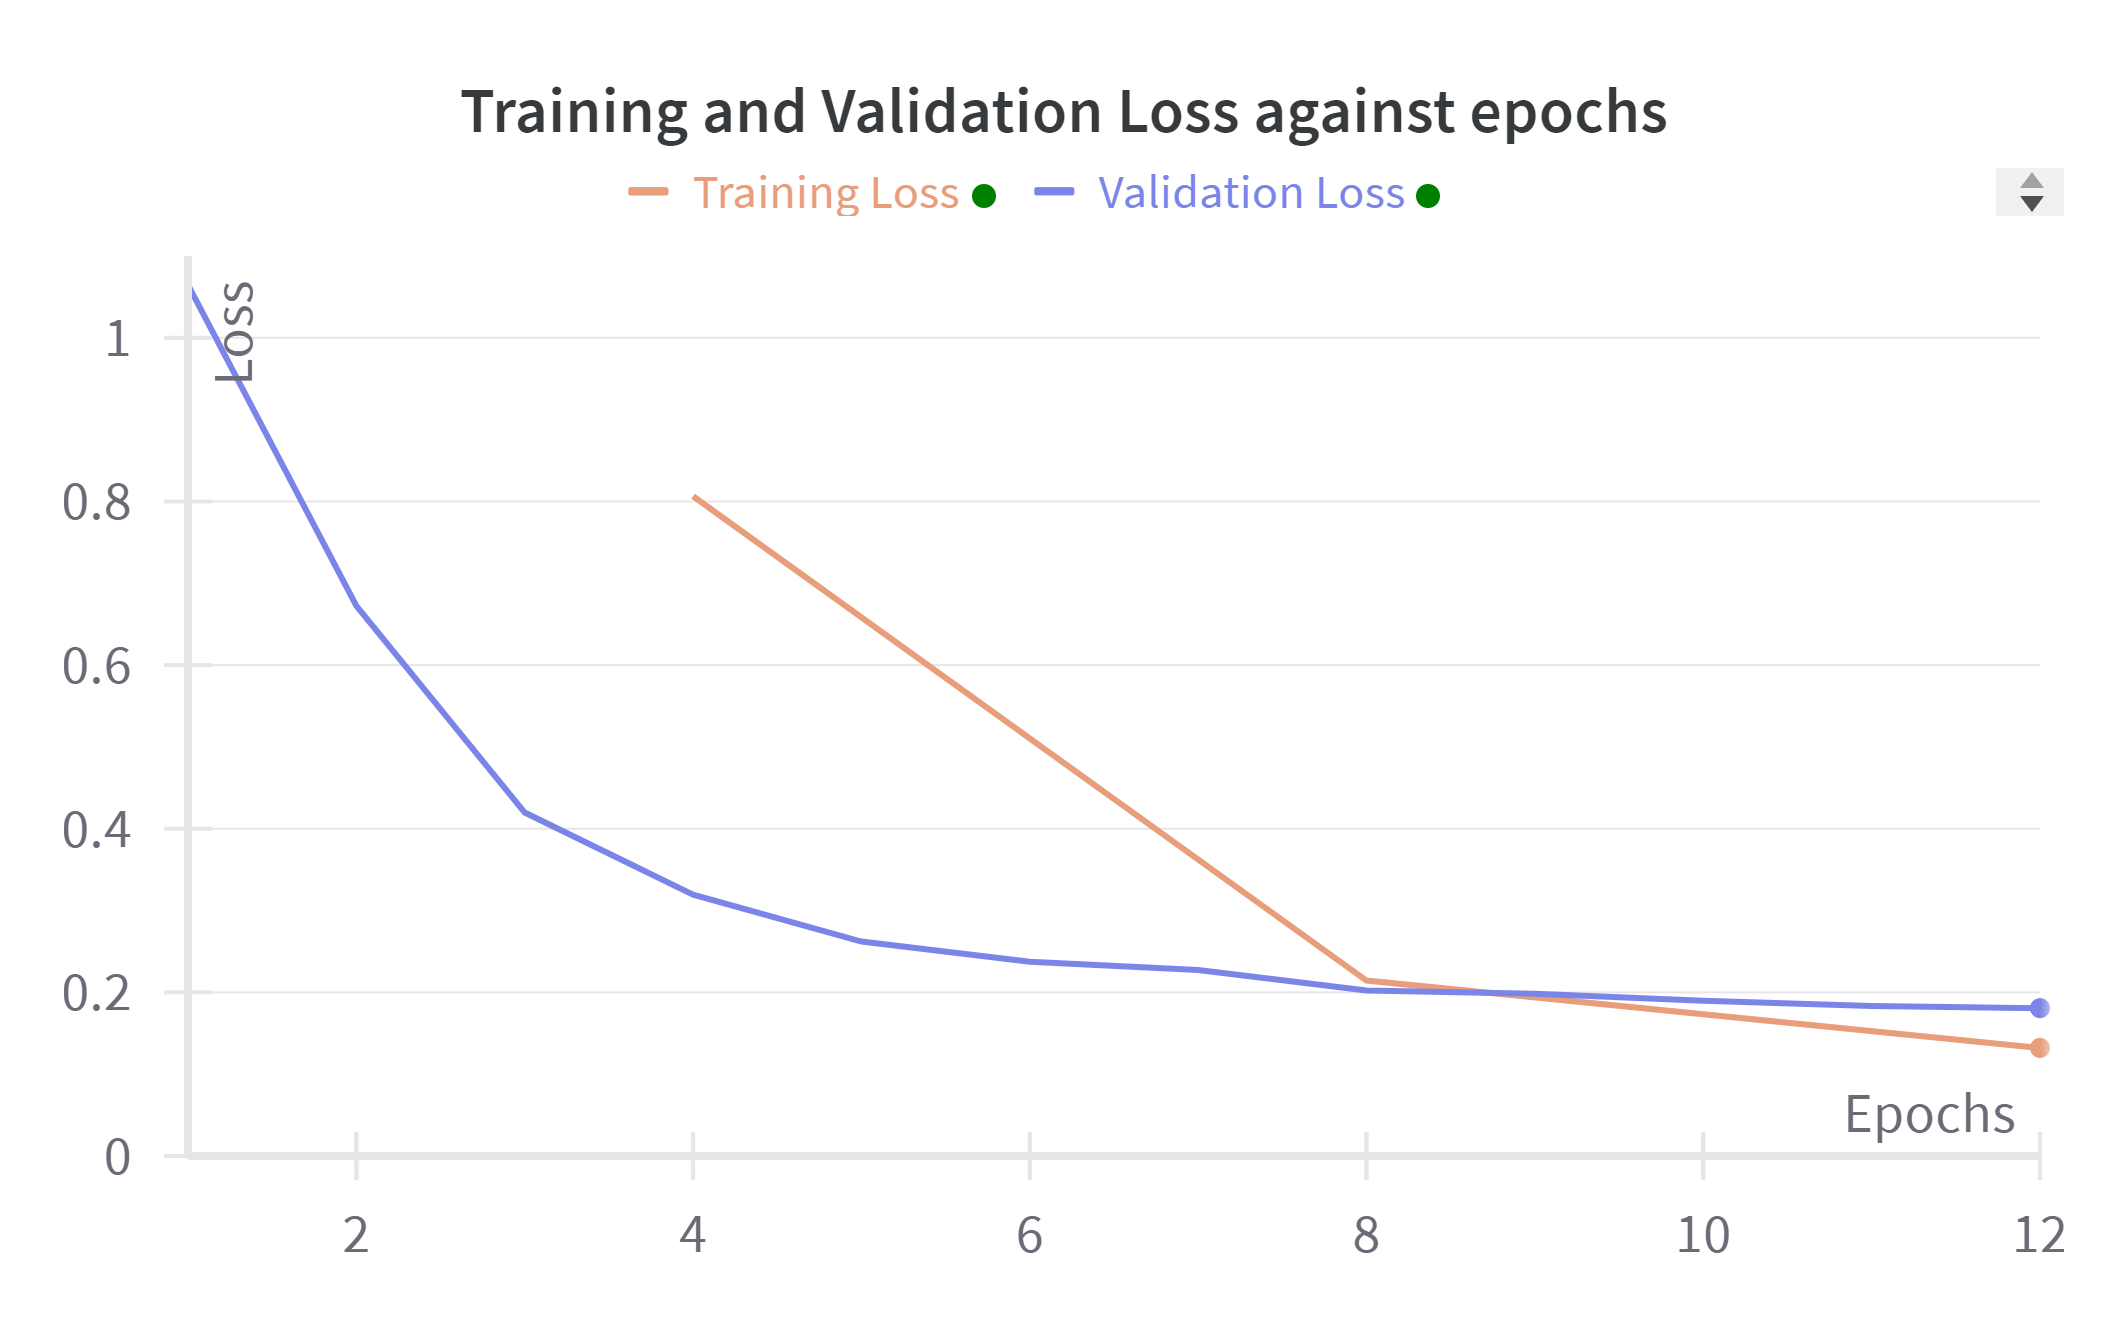
\includegraphics[width=1\linewidth]{Figures/minilm_12_epochs.png}
    \caption{The graph of MiniLM's training and validation loss with 12 epochs}
    \label{fig:minilm_loss_12}
\end{minipage}%
\begin{minipage}{.5\textwidth}
    \centering
    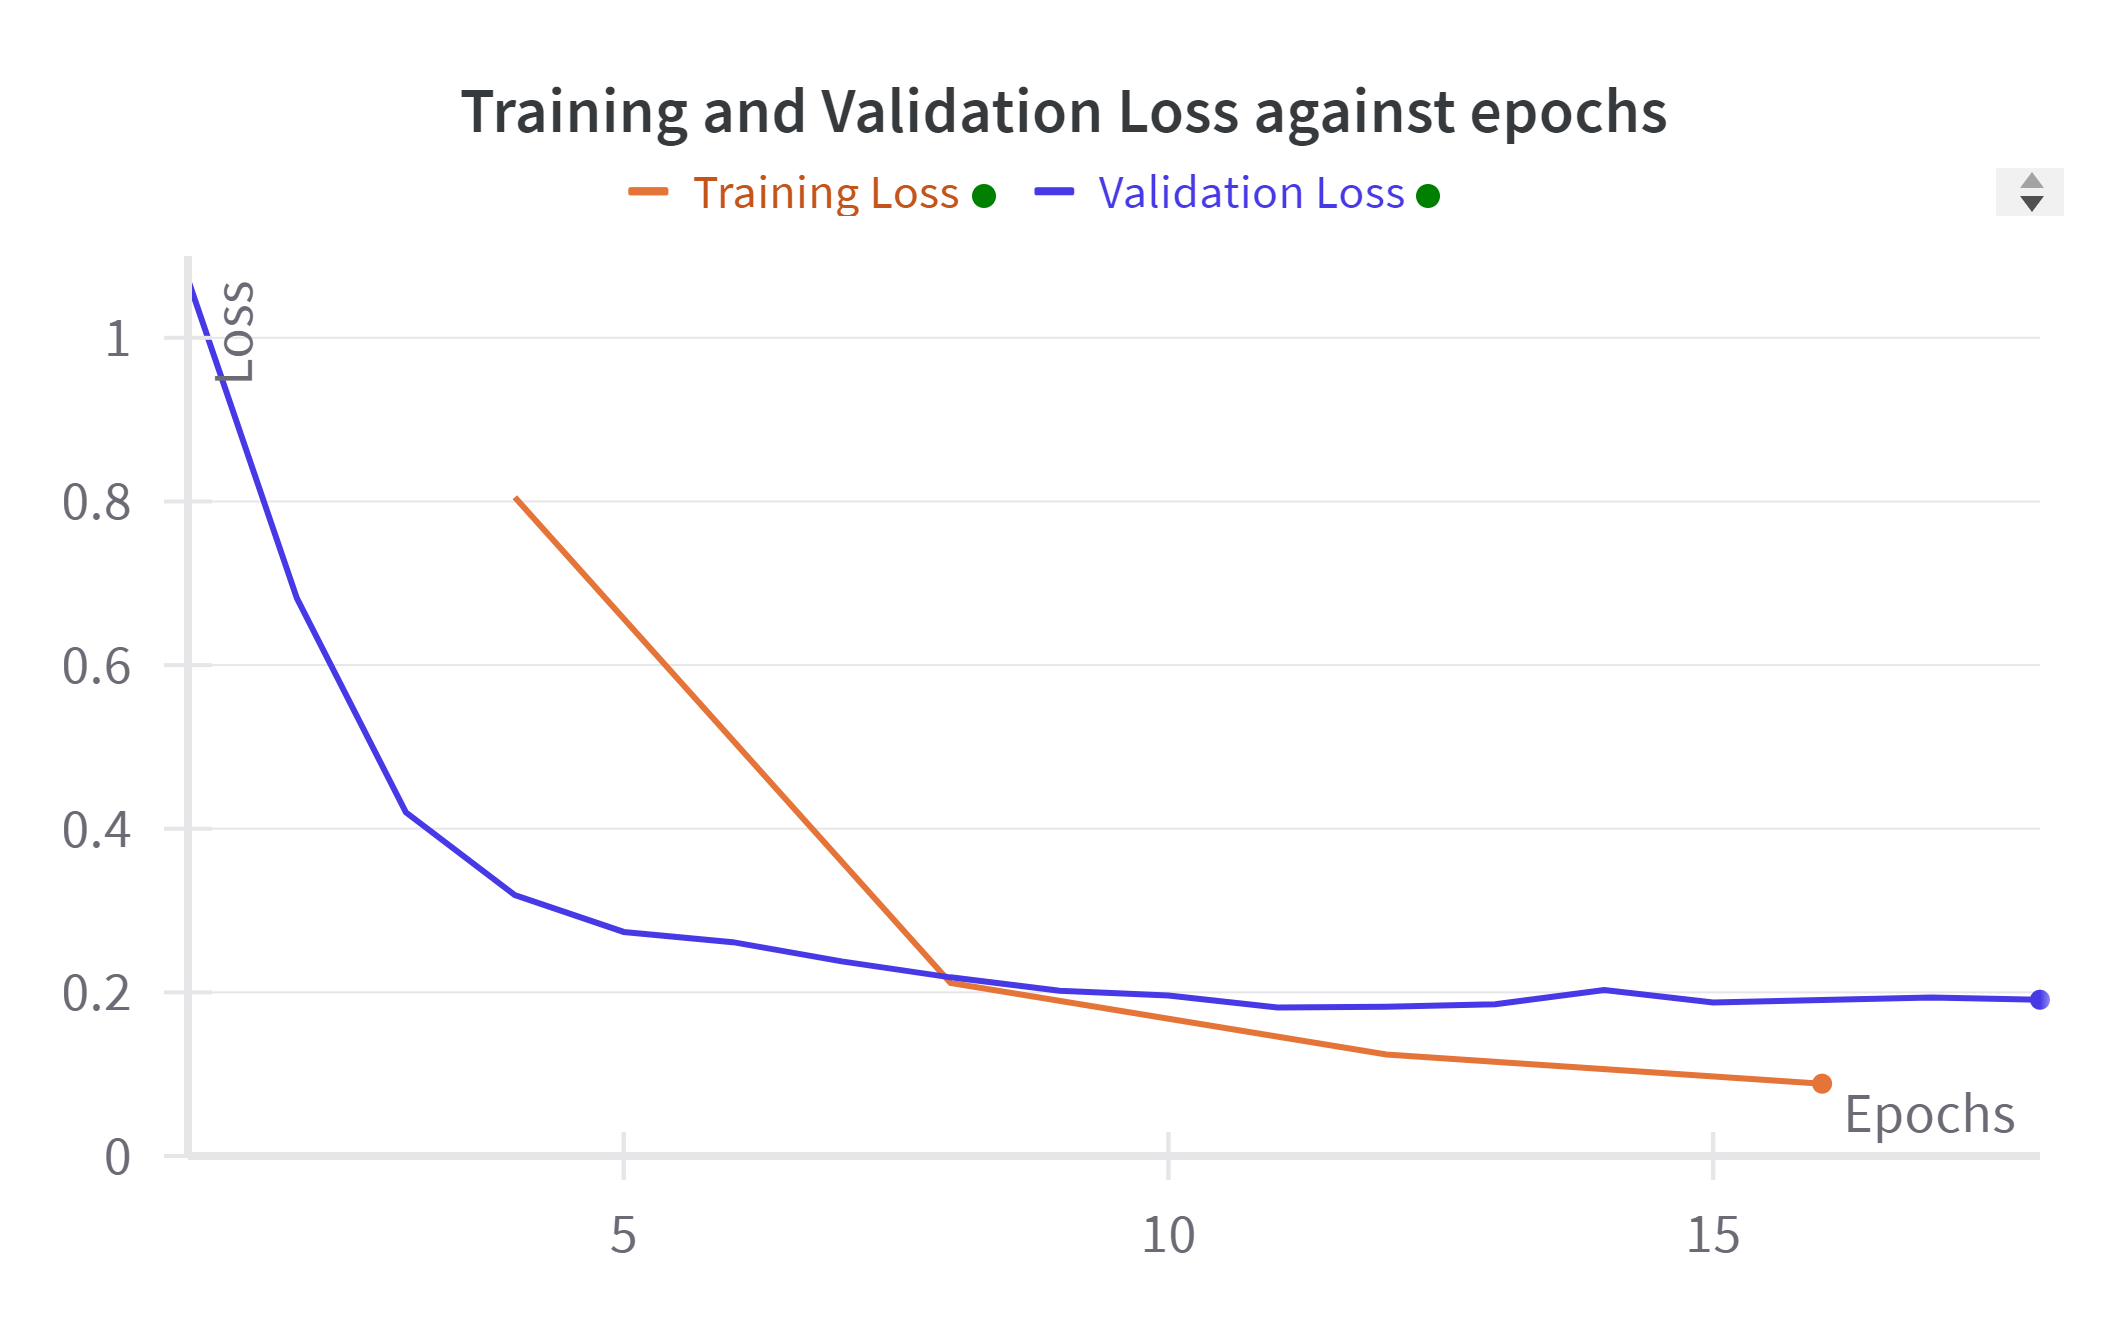
\includegraphics[width=1\linewidth]{Figures/minilm_18_epochs.png}
    \caption{The graph of MiniLM's training and validation loss with 18 epochs}
    \label{fig:minilm_loss_18}
\end{minipage}
\end{figure}

Furthermore, the accuracy and f1-score during training with 12 and 18 epochs are shown in the figure(\ref{fig:minilm_acc_f1_12}) and (\ref{fig:minilm_acc_f1_18}). In both figures, the highest accuracy score reach is 0.93 and the same for f1-score as well. However, there is a small dip for epoch 18, making it 0.928 for both accuracy and f1-score. 

\begin{figure}[h!]
    \centering
    \begin{minipage}{.5\textwidth}
        \centering
        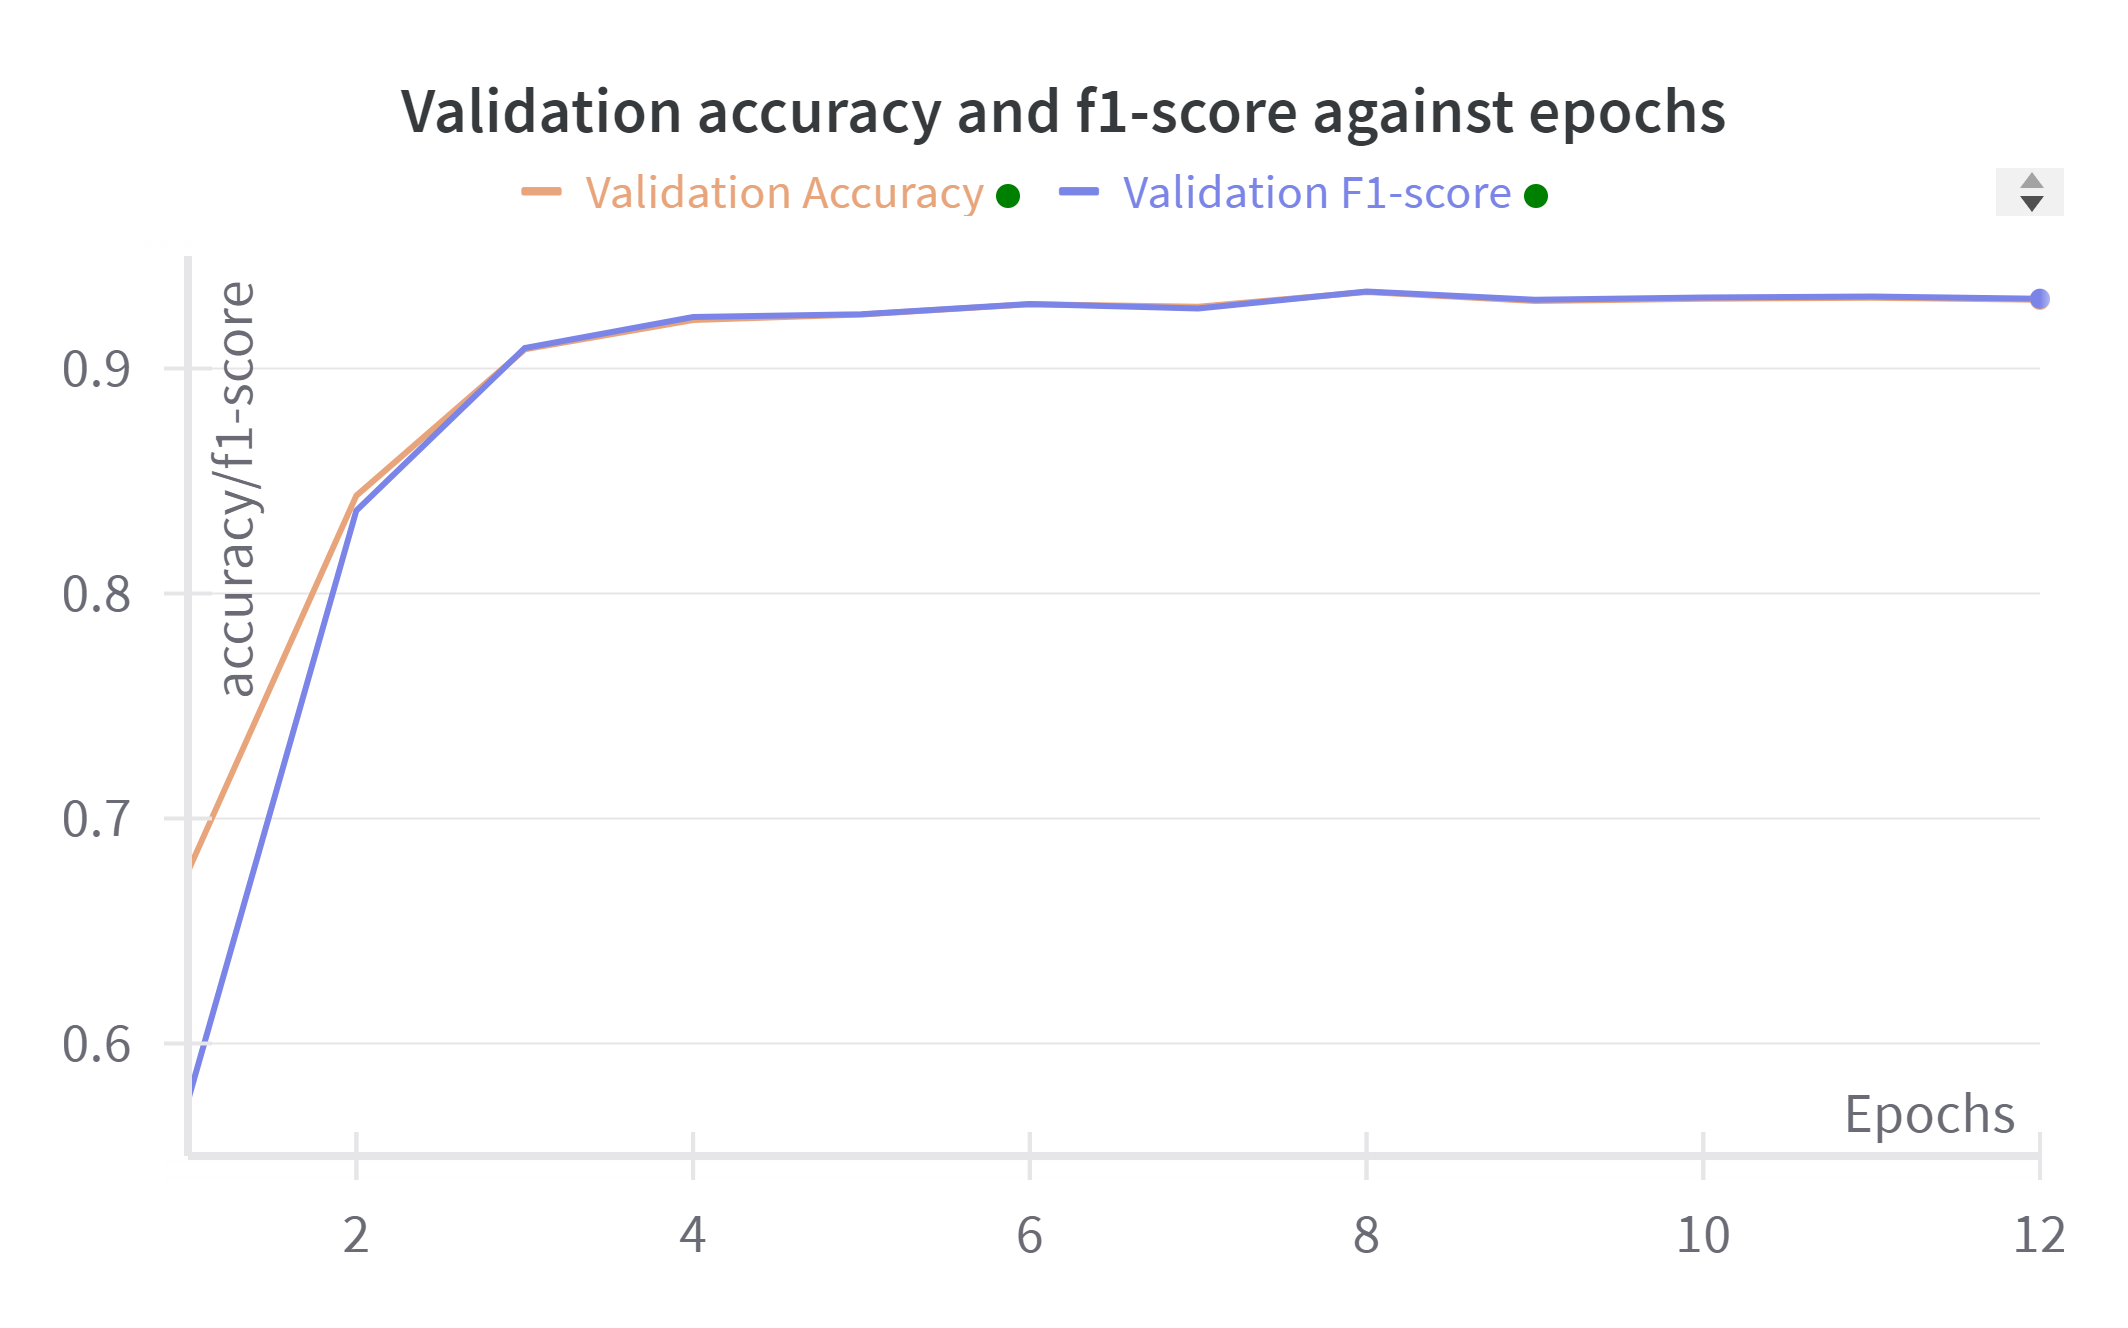
\includegraphics[width=1\linewidth]{Figures/valid_acc_f1_12_epochs_minilm.png}
        \caption{The graph of MiniLM's validation accuracy and f1-score during training with 12 epochs}
        \label{fig:minilm_acc_f1_12}
    \end{minipage}%
    \begin{minipage}{.5\textwidth}
        \centering
        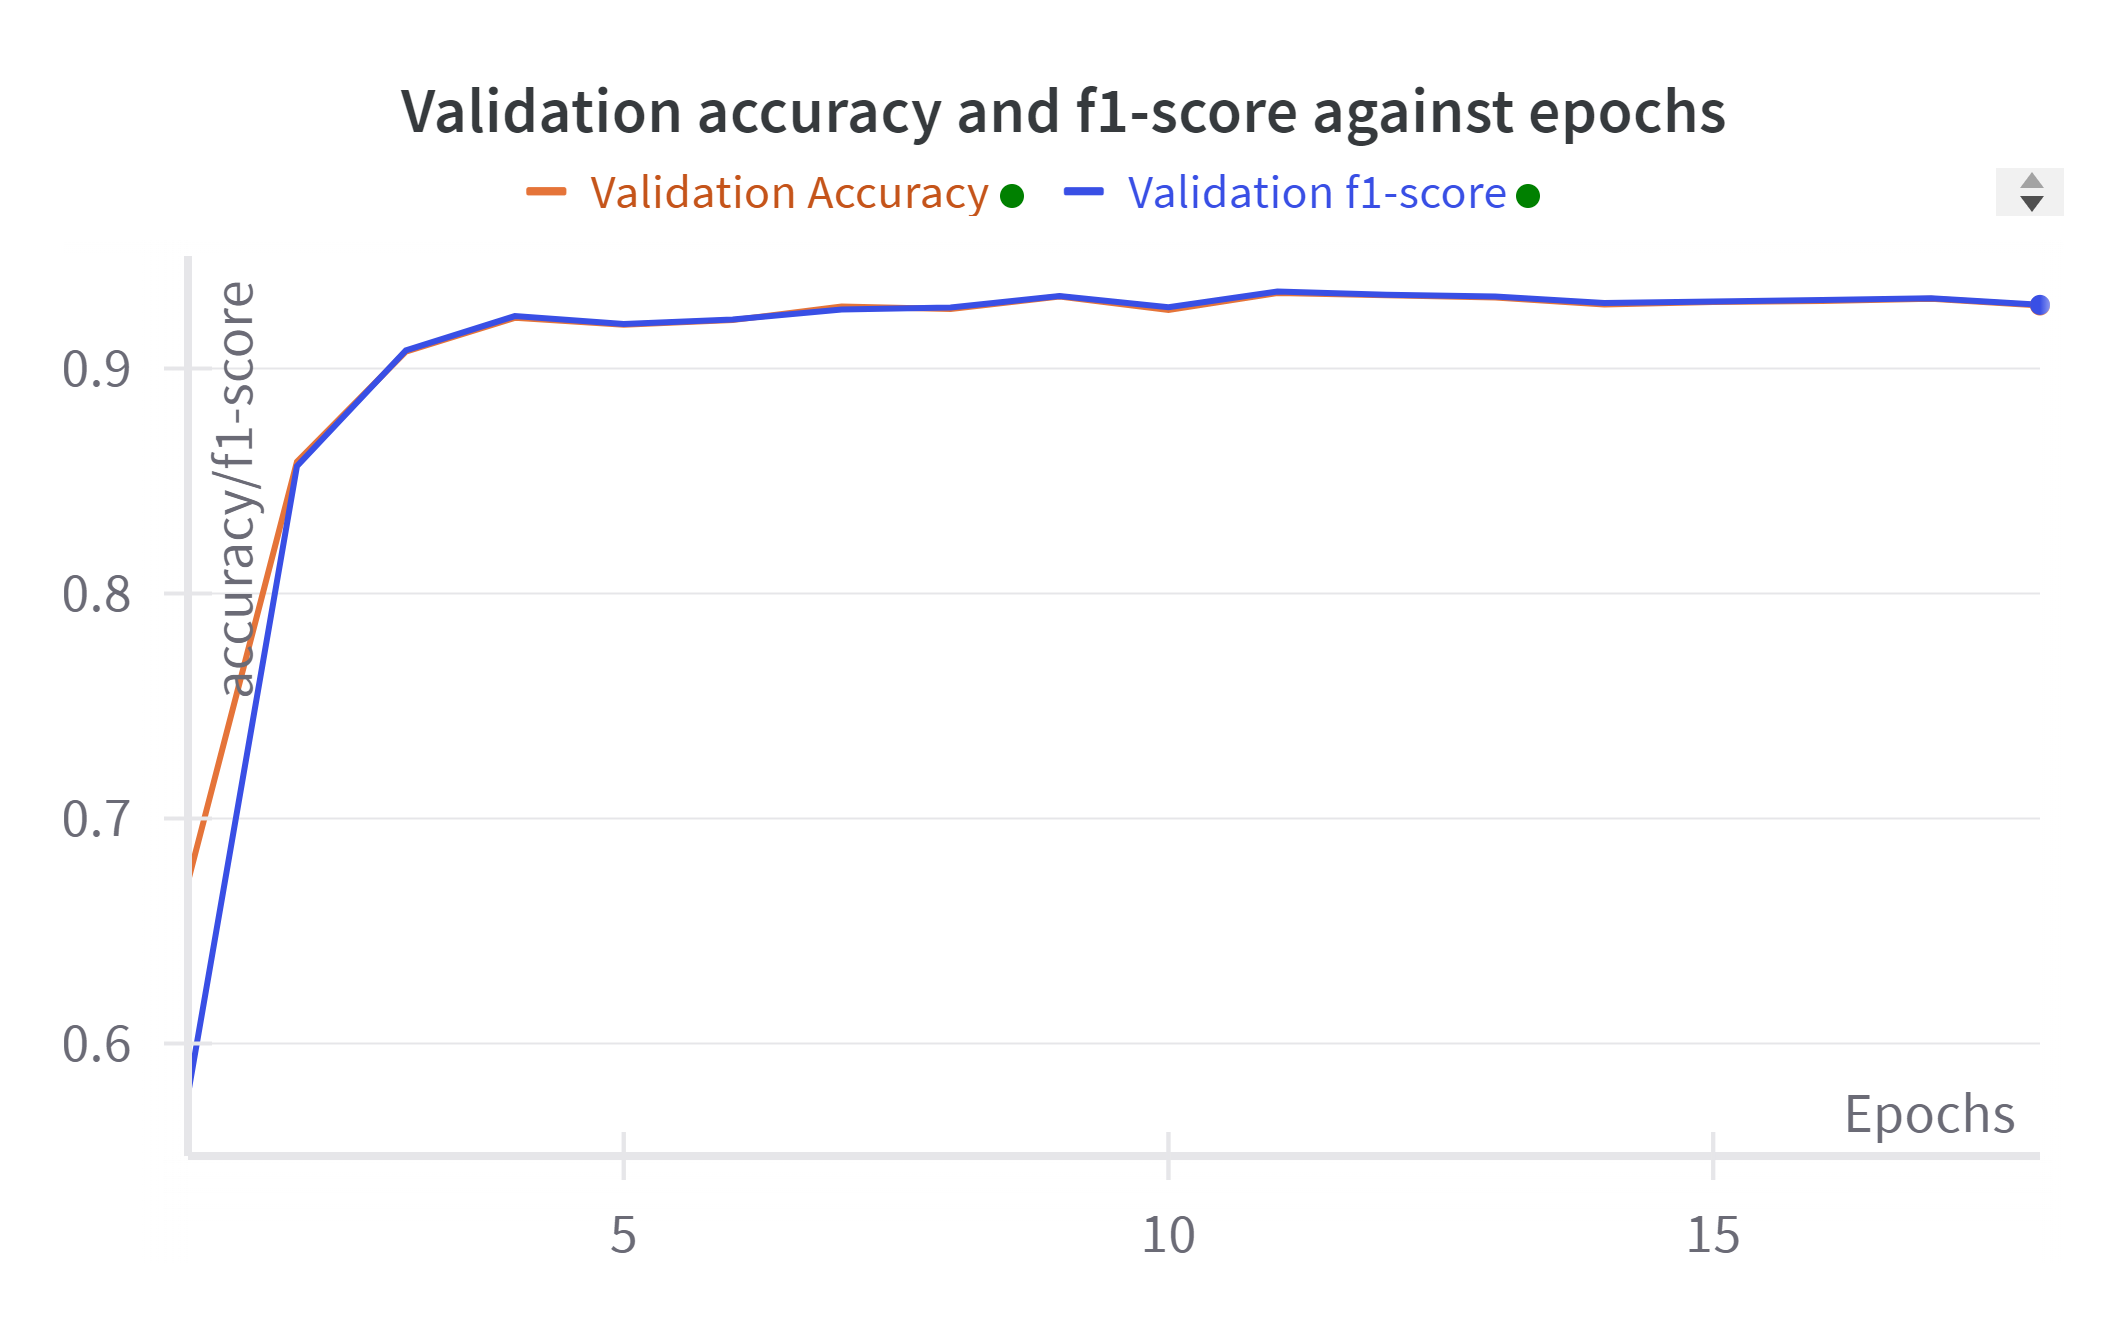
\includegraphics[width=1\linewidth]{Figures/val_acc_f1_18_epochs_minilm.png}
        \caption{The graph of MiniLM's validation accuracy and f1-score during training with 18 epochs}
        \label{fig:minilm_acc_f1_18}
    \end{minipage}
\end{figure}

The table(\ref{tab:overall_metrics}) shows all the average of metrics for each epoch ran. It seems that the numbers of epochs do not affect the performance of the model as there is no big changes in any of the metrics. The best accuracy and f1-score being 0.93 and 0.89 respectively.

\begin{table}[h!]
    \centering
    \begin{tabular}{|c|c|c|c|c|}\hline
          Epochs  & Overall Precision & Overall Recall & Overall F1-score & Overall Accuracy\\\hline
           6 & 0.90 & 0.86 & 0.88 & 0.92\\\hline
           12 & 0.90 & 0.87 & 0.89 & 0.93\\\hline
           18 & 0.90 & 0.87 & 0.88 & 0.93\\\hline
    \end{tabular}
    \caption{The table for the overall values of every metrics in each epoch}
    \label{tab:overall_metrics}
\end{table}

The following diagrams are confusion matrices for each epoch, figure(\ref{fig:conf_6}), (\ref{fig:conf_12}) and (\ref{fig:conf_18}). Overall, the model prediction for "sadness", "joy" and "fear" labels improve as the numbers of epochs increase. The most wrong prediction done for all across the epochs is when the model predicted "joy" but the true label is "love". The prediction improved as the model was trained with more epochs reducing from 55 to 35 at 18 epochs. On the other hand, the increase of label "love" was predicted instead of "joy". It increased from 4 to 17 at epoch 18. 

Nevertheless, the model did well in differentiating positive and negative emotions as "joy" and "love" labels were not predicted too much as "anger", "fear" or "sadness", and vice versa.

\begin{figure}[h!]
    \centering
    \begin{minipage}{.5\textwidth}
        \centering
        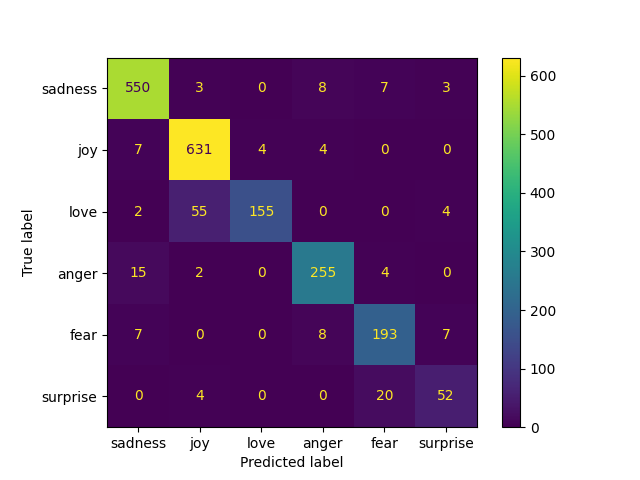
\includegraphics[width=1\linewidth]{Figures/conf_metrix_minilm_6_epochs.png}
        \caption{Confusion Matrix 6 epochs}
        \label{fig:conf_6}
    \end{minipage}%
    \begin{minipage}{.5\textwidth}
        \centering
        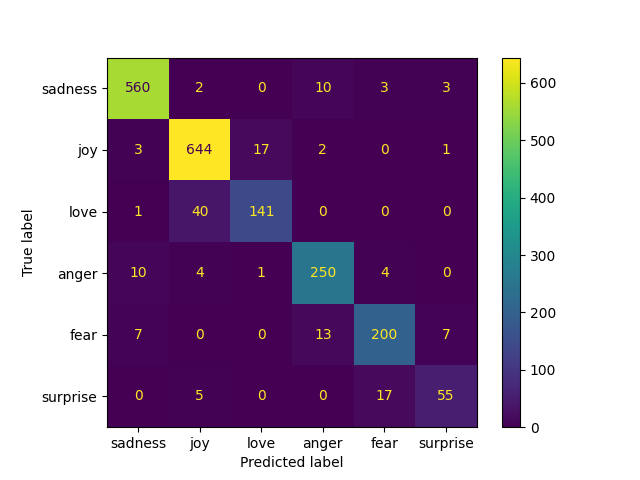
\includegraphics[width=1\linewidth]{Figures/conf_metrix_minilm_12_epochs.png}
        \caption{Confusion Matrix 12 epochs}
        \label{fig:conf_12}
    \end{minipage}
    \begin{minipage}{.5\textwidth}
        \centering
        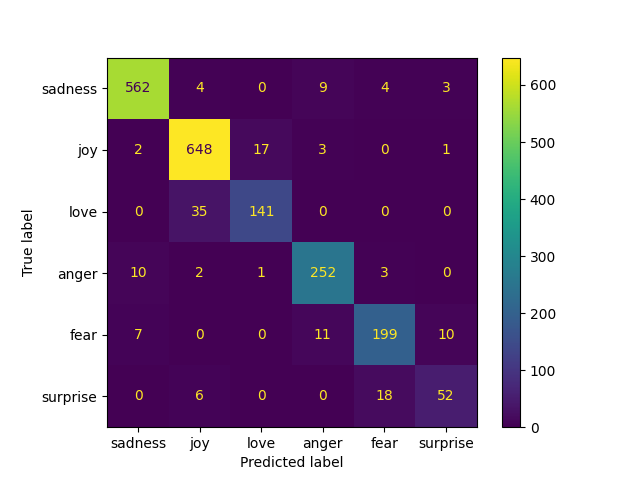
\includegraphics[width=1\linewidth]{Figures/conf_metrix_minilm_18_epochs.png}
        \caption{Confusion Matrix 18 epochs}
        \label{fig:conf_18}
    \end{minipage}%
\end{figure}

\section{RoBERTa}

The zero-shot testing is done for RoBERTa as well and the accuracy was 32\% making it 10 times better than MiniLM. Even so, the predictions the model made is still worse as it only predict either label "joy" or "surprise" making accuracy for "joy", 91\% and 9.1\% for "sadness" label's accuracy. The overall f1-score is around 9\%. This means that RoBERTa is also a model which needs to be fine-tuned before testing the model.

The hyperparameters for training RoBERTa model is the same as MiniLM model. The table of hyperparameters is as listed in table(\ref{tab:hyp_MiniLM}).\bigskip
\bigskip
\bigskip
\bigskip
\begin{figure}[h!]
    \centerline{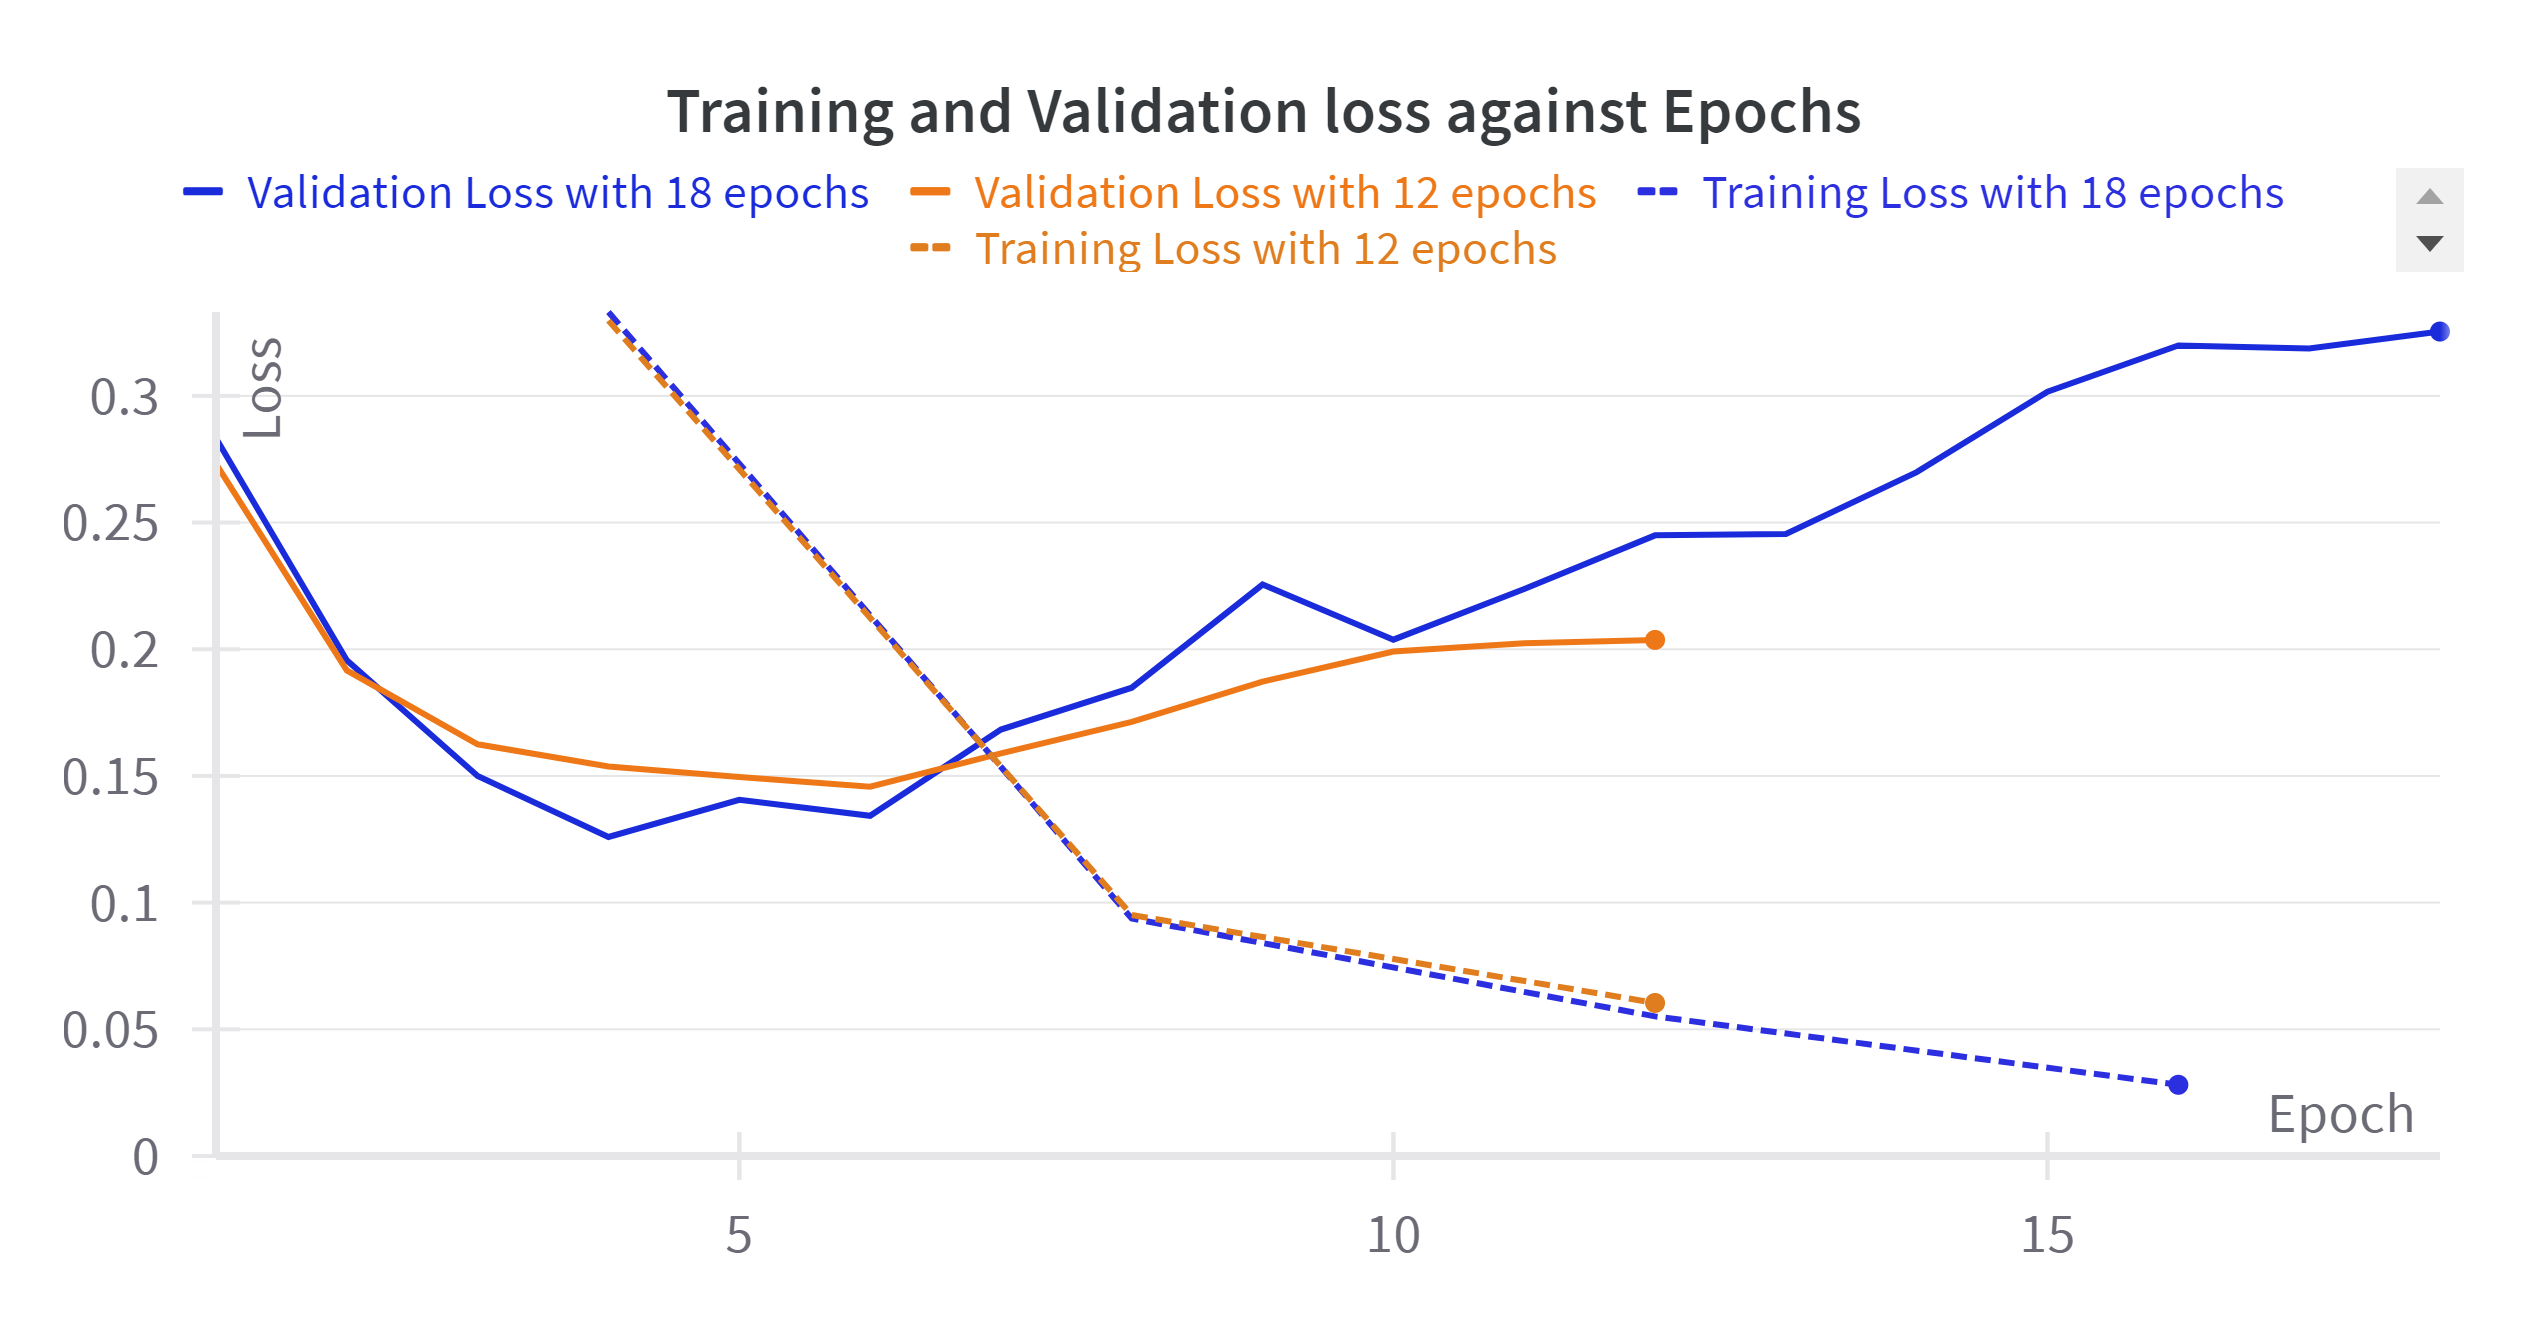
\includegraphics[scale=0.17]{Figures/val_train_loss_12_18 _epochs.png}}
    \caption{The graph for Training and Validation loss for both 12 and 18 epochs across epochs}
    \label{fig:val_train_loss_rob}
\end{figure}

The line graph in the figure(\ref{fig:val_train_loss_rob}) shows the training and validation losses during the training. The training losses are the similar for both epochs and reaching to the lowest of around 0.0281. On the other hand, the validation loss increases as the number of epochs increases and the highest being 0.3254 at 18 epochs. The training loss and validation loss converges as the number of epochs increases which means that the more the model trained, the more it will overfit.

\begin{figure}[h!]
    \centering
    \begin{minipage}{.5\textwidth}
        \centering
        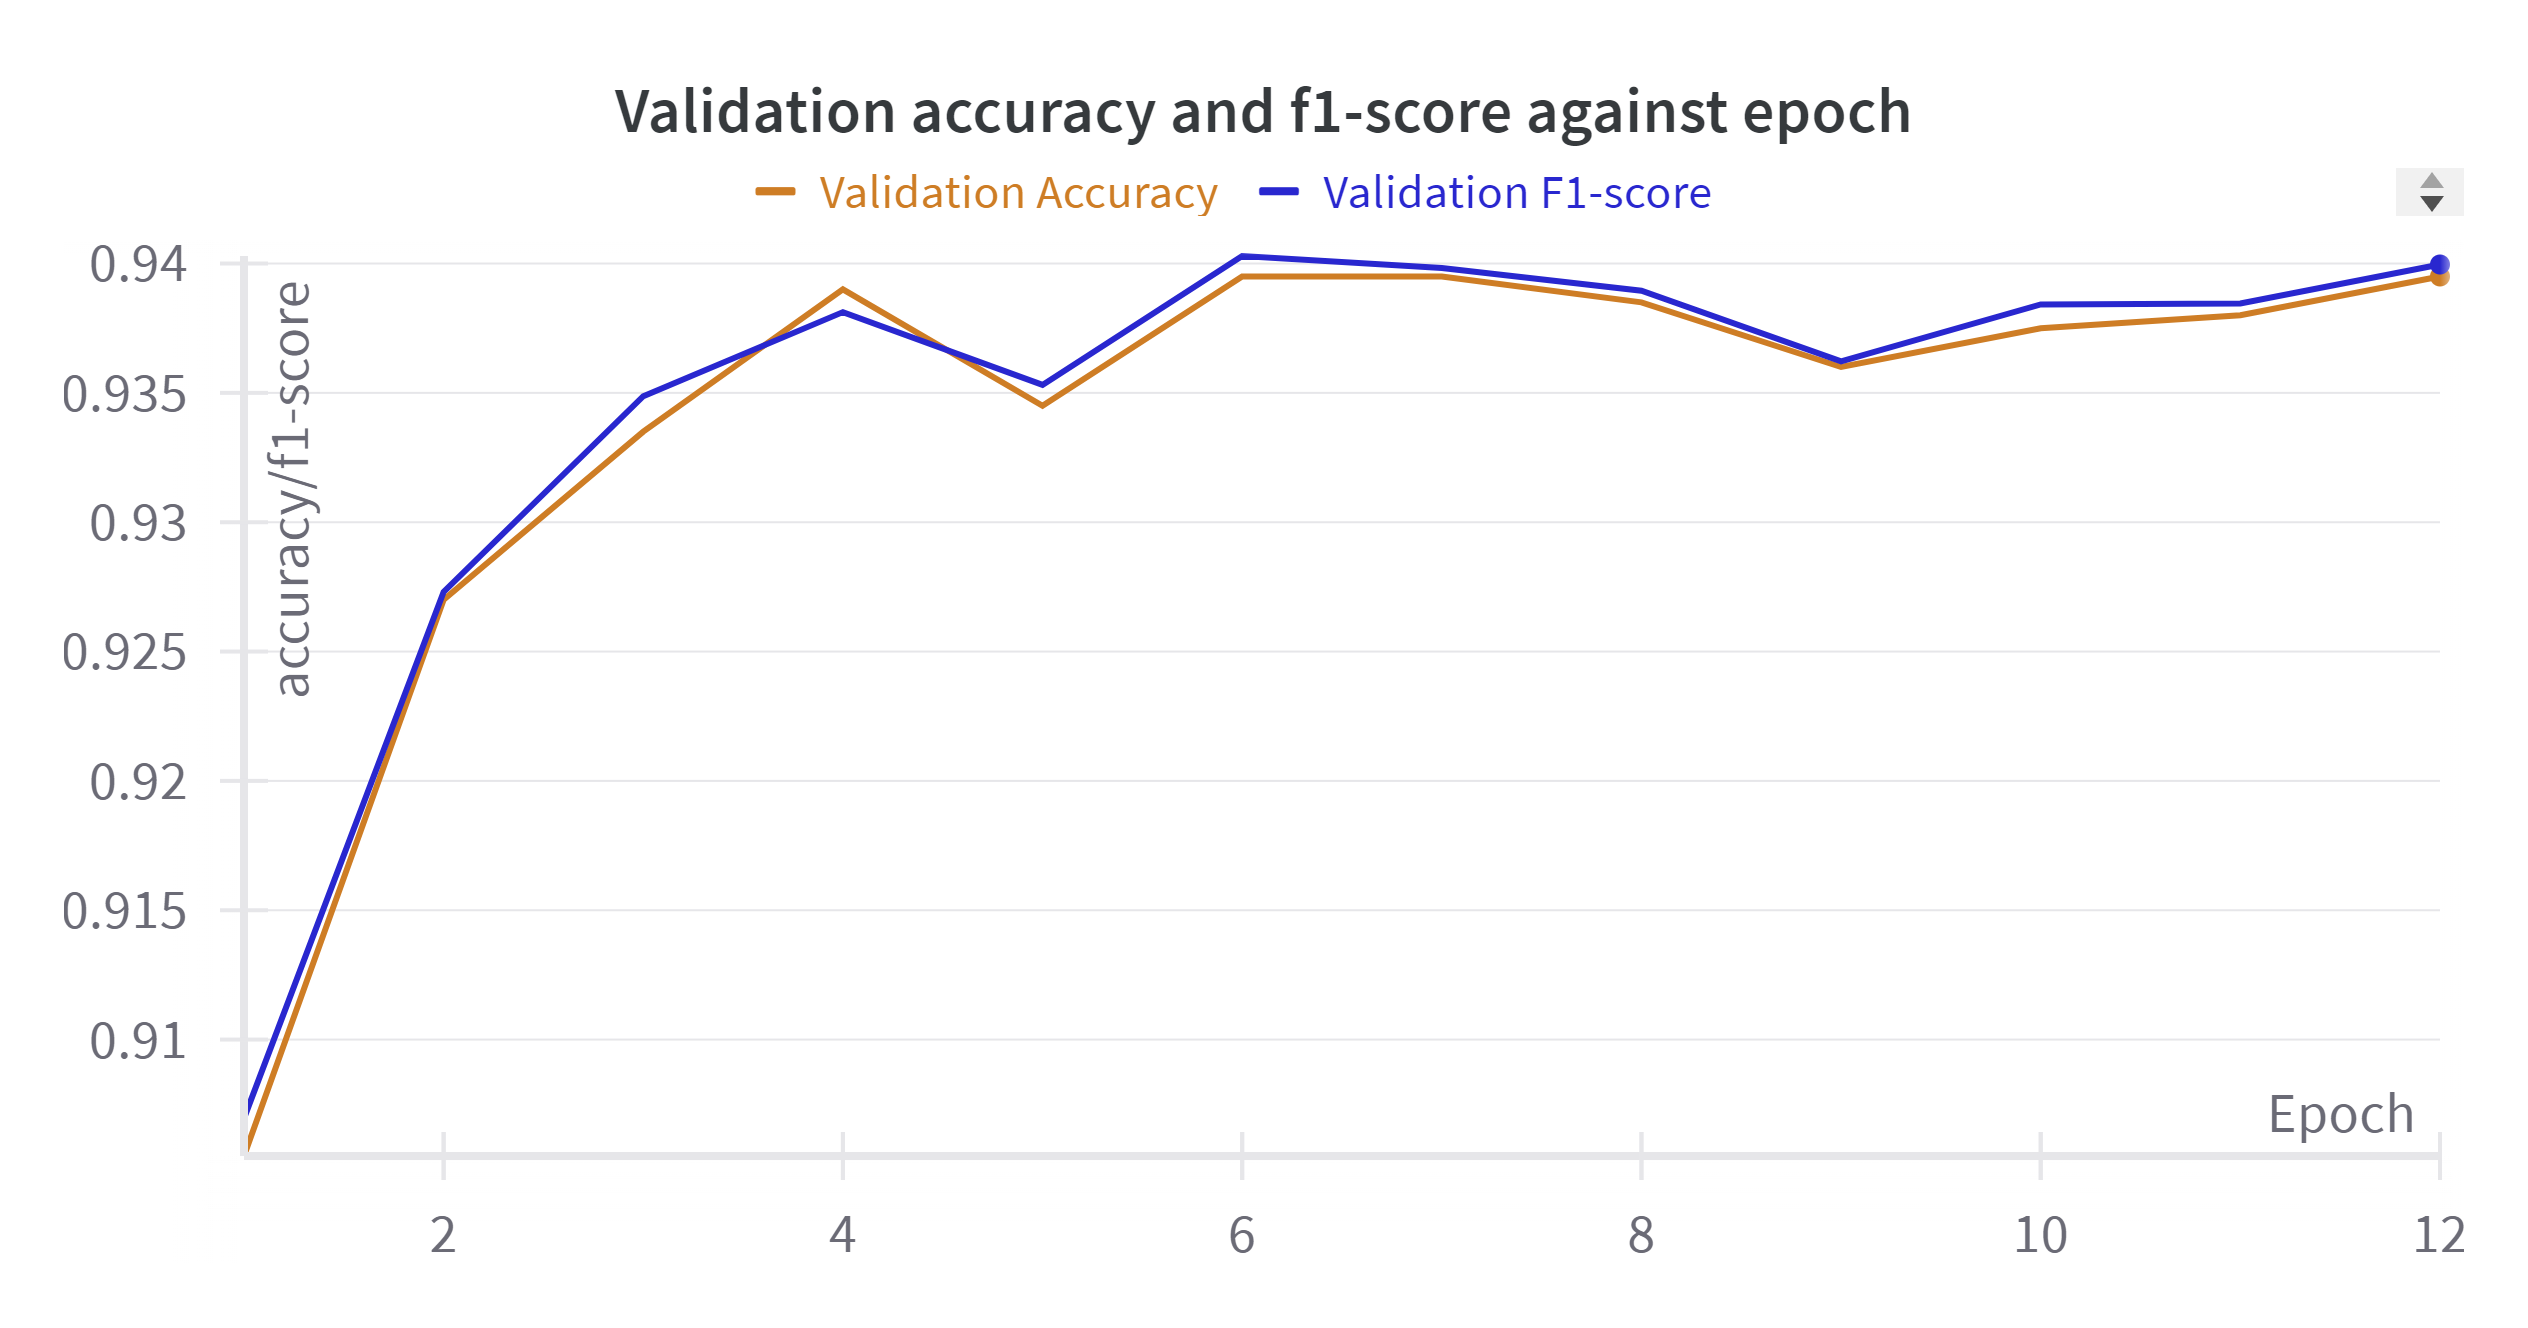
\includegraphics[width=1\linewidth]{Figures/val_ac_f1_12_rob.png}
        \caption{The graph of RoBERTa's validation accuracy and f1-score during training with 12 epochs}
        \label{fig:RoBERTa_acc_f1_12}
    \end{minipage}%
    \begin{minipage}{.5\textwidth}
        \centering
        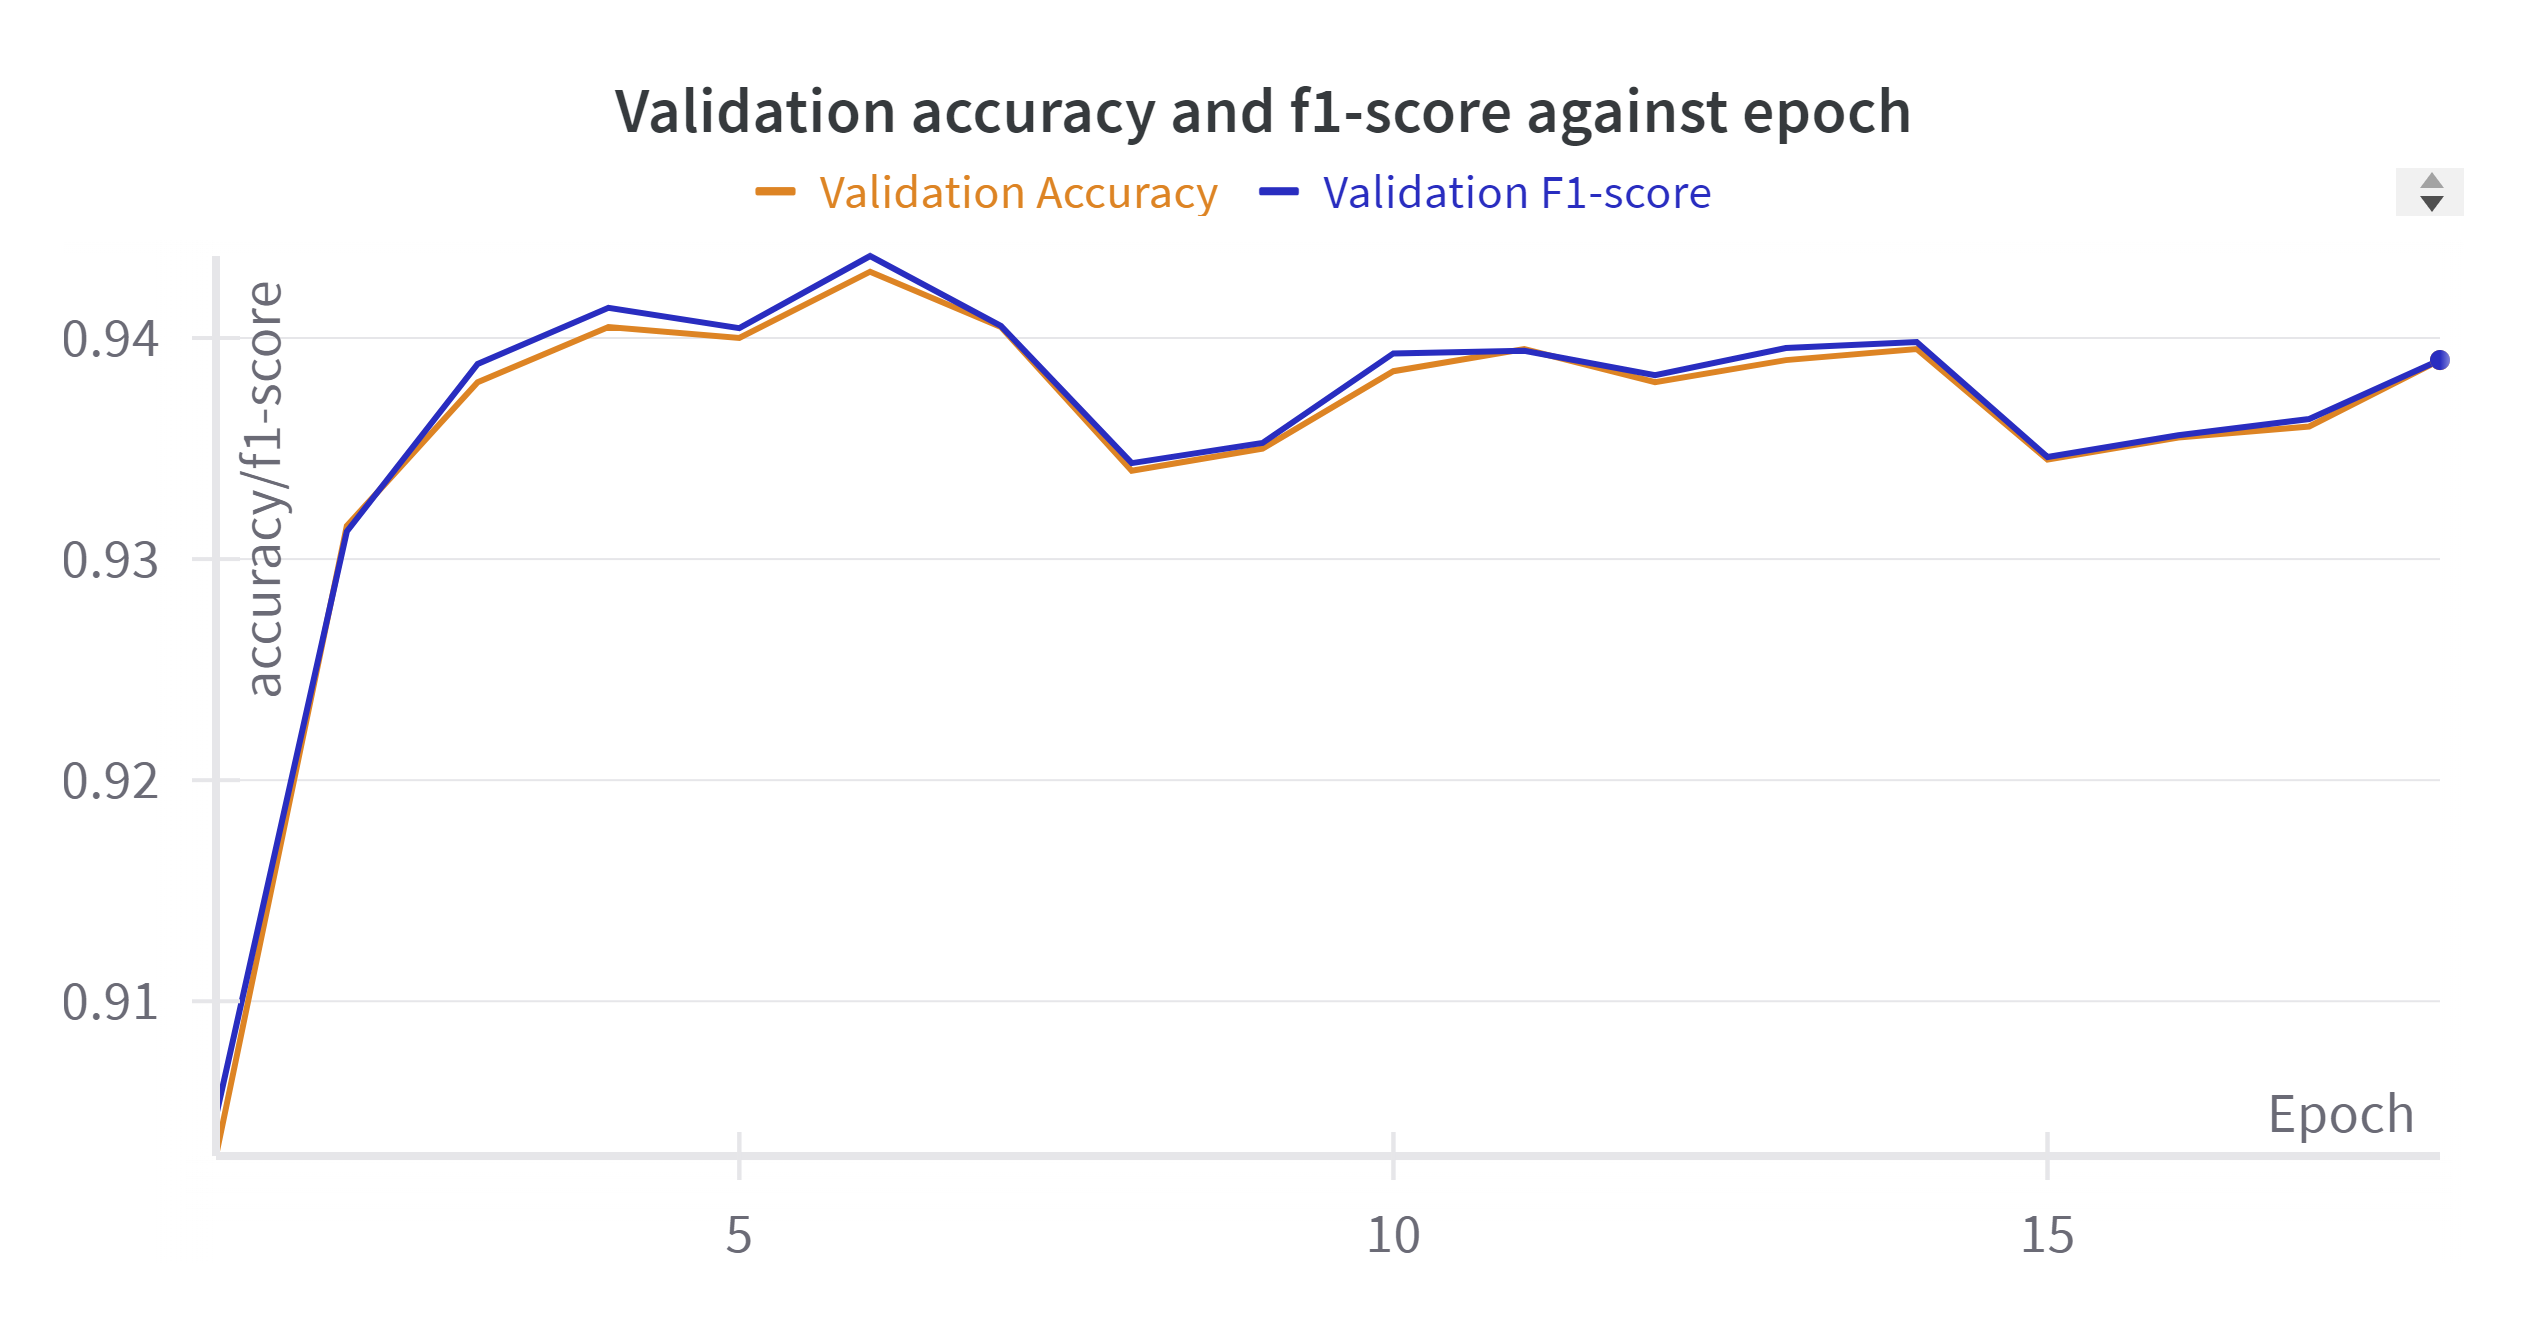
\includegraphics[width=1\linewidth]{Figures/val_ac_f1_18_rob.png}
        \caption{The graph of RoBERTa's validation accuracy and f1-score during training with 18 epochs}
        \label{fig:RoBERTa_acc_f1_18}
    \end{minipage}
\end{figure}

The Figure(\ref{fig:RoBERTa_acc_f1_12}) and (\ref{fig:RoBERTa_acc_f1_18}) show that accuracy and f1-score are similar across epochs. Both of the graphs also shows that the accuracy and f1-score could go as high as around 94\%.  

\begin{table}[h!]
    \centering
    \begin{tabular}{|c|c|c|c|c|}\hline
          Epochs  & Overall Precision & Overall Recall & Overall F1-score & Overall Accuracy\\\hline
           6 & 0.87 & 0.9 & 0.88 & 0.927\\\hline
           12 &  0.88 & 0.9 & 0.89 & 0.929\\\hline
           18 & 0.89 & 0.9 & 0.89 & 0.93\\\hline
    \end{tabular}
    \caption{The table for the overall values of every metrics in each epoch}
    \label{tab:overall_metrics_rob}
\end{table}

The table(\ref{tab:overall_metrics_rob}) shows that the best epochs out of all three is epoch 18 as all overall metrics are higher than the other two.

\begin{figure}[h!]
    \centering
    \begin{minipage}{.5\textwidth}
        \centering
        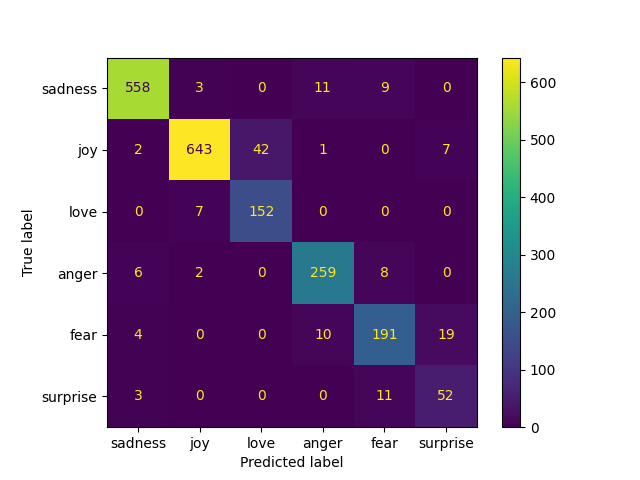
\includegraphics[width=1\linewidth]{Figures/conf_metrix_roberta_6_epochs.png}
        \caption{Confusion Matrix 6 epochs}
        \label{fig:conf_6_rob}
    \end{minipage}%
    \begin{minipage}{.5\textwidth}
        \centering
        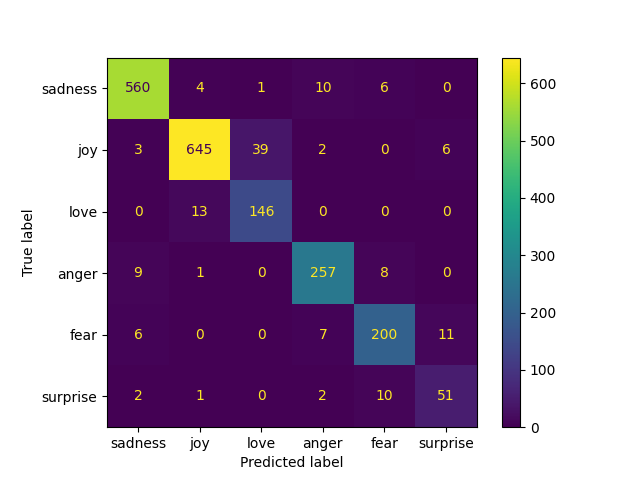
\includegraphics[width=1\linewidth]{Figures/conf_metrix_roberta_12_epochs.png}
        \caption{Confusion Matrix 12 epochs}
        \label{fig:conf_12_rob}
    \end{minipage}
    \begin{minipage}{.5\textwidth}
        \centering
        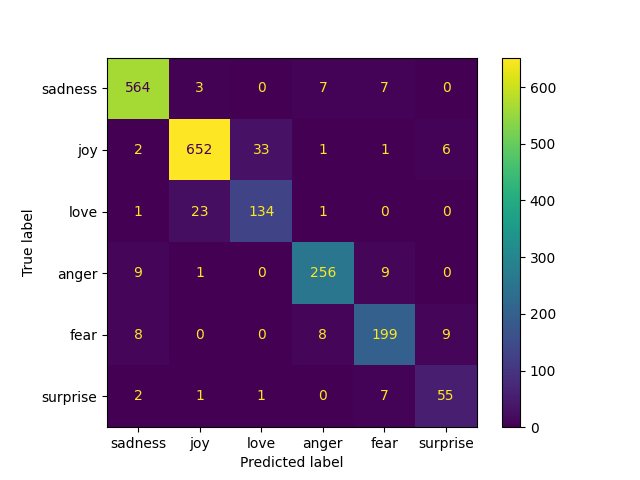
\includegraphics[width=1\linewidth]{Figures/conf_metrix_roberta_18_epochs.png}
        \caption{Confusion Matrix 18 epochs}
        \label{fig:conf_18_rob}
    \end{minipage}%
\end{figure}

The model is good at classifying the labels such as "sadness", "joy", "anger" and "surprise" as the number for each label correctly predicted increases. The diagrams of confusion matrix for each number of epochs can be seen in figure(\ref{fig:conf_6_rob}), (\ref{fig:conf_12_rob}) and (\ref{fig:conf_18_rob}). The label "joy" and "love" was mixed up, similar to MiniLM model however, the model predicted "joy" instead of "love" more as the number of epochs increased. This maybe because "joy" and "love" both are emotions that are similar to each other and most of the time, they are expressed together.

\section{GPT-2}
As for GPT-2, the prediction's accuracy is a bit better than the models above when it was tested before the training. The accuracy overall for it is 34.6\% however, the label that is mainly predicted is "joy". The f1-score is 9\%. Thus, GPT-2 is also the model which is not good for zero-shot testing.
\bigskip
\bigskip
\bigskip
\bigskip
\bigskip
\bigskip
\bigskip

\textbf{Hyperparameters:}

\begin{table}[h!]
    \centering
    \begin{tabular}{c|c}
        Hyperparameters & Values\\\hline
        Loss Func & CrossEnthropy (default)\\
        Optimiser & adamW\_torch (default)\\
        Learning rate & 2e-5\\
        Batch size & 1\\
        Weight Decay & 0.01\\
    \end{tabular}
    \caption{Hyperparameters for GPT-2 model}
    \label{tab:hyp_GPT}
\end{table}

The table(\ref{tab:hyp_GPT}) shows the hyperparameters for GPT-2's training arguments. The batch size is 1 as more than one uses up the memory that it make the model not be able to train. The model is also only train for 2 epochs as it will take more than 8 hours if it was trained on Google Colab which has the limited GPU memory therefore GPU ran out before it is fully trained. If it was locally trained it took nearly a day. Thus, training 2 epochs will be optimal option for GPT-2 model. 

The model training loss started off with 5 and gradually lower in each logging steps within each epoch and at the end reaches to around 0.479 and as for validation loss, the model started off with around 0.298 when it was logged and ended with about 0.246. The model did not seem to overfit during the training with 2 epochs. However, it cannot be said if it trained for more than 2 epochs.

\begin{table}[h!]
    \centering
    \begin{tabular}{|c|c|c|c|c|}\hline
          Epochs  & Overall Precision & Overall Recall & Overall F1-score & Overall Accuracy\\\hline
           2 & 0.89 & 0.88 & 0.88 & 0.931\\\hline
    \end{tabular}
    \caption{The table for the overall values of every metrics in each epoch}
    \label{tab:overall_metrics_gpt2}
\end{table}

\begin{table}[h!]
    \centering
    \begin{tabular}{c|c}
       Labels  & Accuracy\\\hline
        surprise & 0.727\\
        fear & 0.866\\
        joy & 0.967\\
        anger & 0.927\\
        love & 0.805\\
        sadness & 0.972\\
    \end{tabular}
    \caption{Accuracy for each label}
    \label{tab:acc_each_labels}
\end{table}

\begin{table}[h!]
    \centering
    \begin{tabular}{c|c|c|c}
         & Precision & Recall & F1-score\\\hline
         anger & 0.93 & 0.93 & 0.96 \\
         fear & 0.91 & 0.87 &  0.78 \\
         joy & 0.94 & 0.97 & 0.79 \\
         love & 0.88 & 0.81 & 0.83\\
         sadness & 0.96 & 0.97 & 0.83\\
         surprise & 0.72 & 0.73 & 0.83\\
    \end{tabular}
    \caption{Precision, recall and f1-score for each label}
    \label{tab:class_rep_gpt2}
\end{table}

Nonetheless, the model did well with emotion classification task as its overall accuracy is 93\% and macro average f1-score of 88\% with just 2 epochs of training. All the accuracies for each label is mostly above 80\% with an exception to "surprise" label which has an accuracy of 72.7\%. It was the same for f1-score of each labels as well. The result can be seen in the table(\ref{tab:overall_metrics_gpt2}), (\ref{tab:acc_each_labels}) and (\ref{tab:class_rep_gpt2}) above.

\begin{figure}[h!]
    \centerline{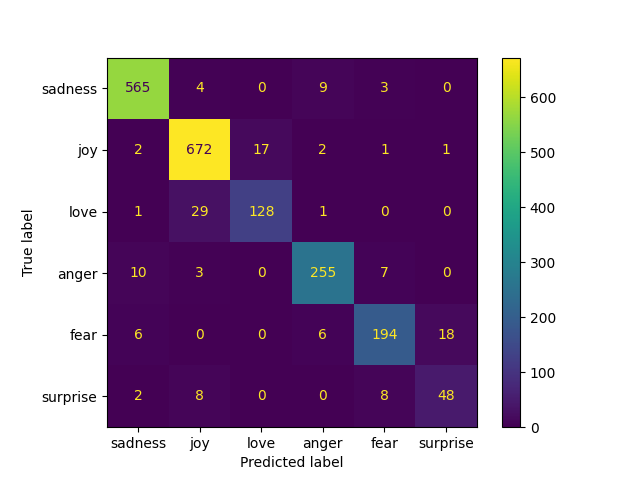
\includegraphics[scale=0.6]{Figures/conf_metrix_gpt2_2_epochs.png}}
    \caption{Confusion Matrix for GPT-2 model with 2 epochs}
    \label{fig:conf_matrix_gpt2}
\end{figure}

Furthermore, the confusion matrix can be seen in figure(\ref{fig:conf_matrix_gpt2}). The most mistake that the model make is the same as MiniLM model. The model was predicting "joy" label when the true label is "love" the same mistake is done in the opposite but a bit less for it. Another mistake that it make is predicting label "surprise" when it should be the label "fear". 

\section{Llama2}

Llama2 is the biggest model that this project has done in terms of parameters and weights. Therefore, I was only able to do one training for Llama2. Firstly, the zero-shot testing was done like all the models that the project implemented. The overall accuracy is the best out of all the models, which is 49.4\%. Which is also the same for overall f1-score with 33\%, it can be seen in table(\ref{tab:overall_metrics_llama2}). However, it predicted outside the range of the labels such as "angst", "disgust", "i guess feelings" and some numbers. The number of samples predicted such labels are 37.

\begin{table}[h!]
    \centering
    \begin{tabular}{|c|c|c|c|c|}\hline
          Epochs  & Overall Precision & Overall Recall & Overall F1-score & Overall Accuracy\\\hline
           zero-shot & 0.43 & 0.34 & 0.33 & 0.494\\\hline
           3 & 0.05 & 0.17 & 0.08 & 0.290\\\hline
    \end{tabular}
    \caption{The table for the overall values of every metrics in zero-shot testing and 3 epochs}
    \label{tab:overall_metrics_llama2}
\end{table}

\begin{table}[h!]
    \centering
    \begin{tabular}{c|c|c}
       Labels  & Accuracy for zero-shot & Accuracy for 3 epochs\\\hline
        surprise & 0.167 & 1\\
        fear & 0.080 &  0\\
        joy & 0.167 & 0 \\
        anger & 0.516 &  0\\
        love & 0.415 & 0 \\
        sadness & 0.706 &  0\\
    \end{tabular}
    \caption{Accuracy for each label both zero-shot and 3 epochs training}
    \label{tab:acc_each_labels_llama2}
\end{table}

\begin{table}[h!]
    \centering
    \begin{tabular}{c|c|c|c}
         & Precision & Recall & F1-score\\\hline
         anger & 0.44 & 0.52 & 0.47 \\
         fear & 0.78 & 0.08 &  0.15 \\
         joy & 0.74 & 0.49 & 0.59 \\
         love & 0.26 & 0.42 & 0.32\\
         sadness & 0.48 & 0.71 & 0.57\\
         surprise & 0.31 & 0.17 & 0.22\\
    \end{tabular}
    \caption{Precision, recall and f1-score for each label}
    \label{tab:class_rep_llama2}
\end{table}
\bigskip
\bigskip
\bigskip
\bigskip
\bigskip
\bigskip
\bigskip
Table(\ref{tab:acc_each_labels_llama2}) and (\ref{tab:class_rep_llama2}) show that the accuracy, precision, recall and f1-score of each label. The best accuracy is the label "sadness" as well as the highest recall, and the best f1-score is the label "joy". The highest precision is the label "fear".

\begin{figure}[h!]
    \centerline{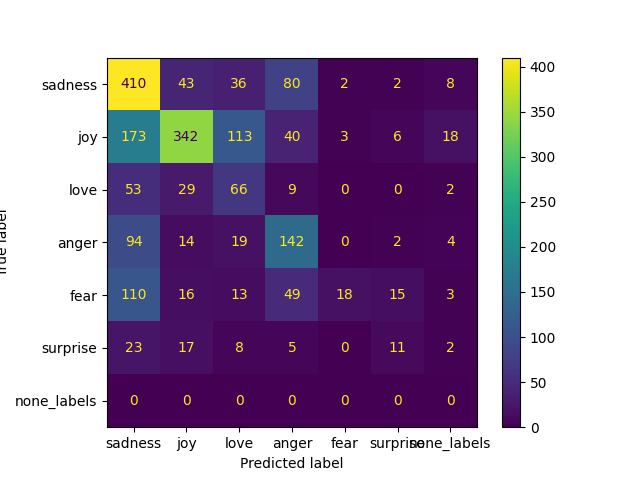
\includegraphics[scale=0.6]{Figures/conf_metrix_llama2_no_epochs.png}}
    \caption{Confusion Matrix for Llama2 zero-shot}
    \label{fig:conf_matrix_llama2}
\end{figure}

The none\_labels in figure(\ref{fig:conf_matrix_llama2}) shows that the labels which are not predicted within the bounds of the given labels. It can be seen that most of the labels should have predicted as "joy" but predicted some random words, number or beginning part of sentences. Apart from them, the model is still not the best at detecting most of the testing sample incorrectly. However, it seemed that it mostly did not predict negative emotions as positive and vice versa.